% Created by tikzDevice version 0.12.6 on 2026-05-17 18:10:12
% !TEX encoding = UTF-8 Unicode
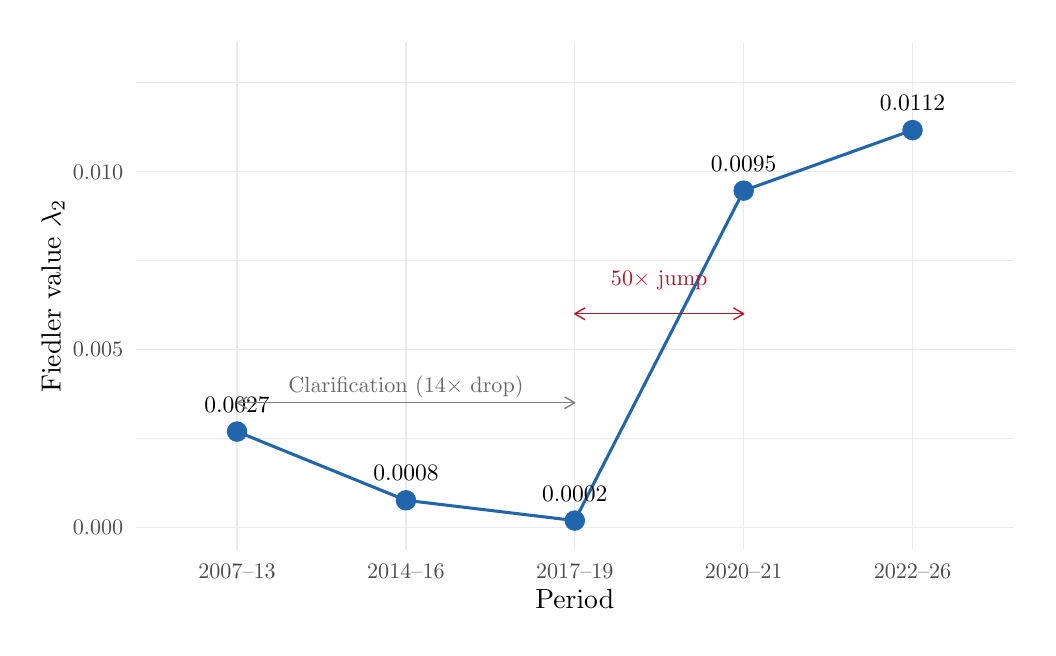
\begin{tikzpicture}[x=1pt,y=1pt]
\definecolor{fillColor}{RGB}{255,255,255}
\path[use as bounding box,fill=fillColor,fill opacity=0.00] (0,0) rectangle (361.35,216.81);
\begin{scope}
\path[clip] (  0.00,  0.00) rectangle (361.35,216.81);
\definecolor{fillColor}{RGB}{255,255,255}

\path[fill=fillColor] ( -0.00,  0.00) rectangle (361.35,216.81);
\end{scope}
\begin{scope}
\path[clip] ( 39.05, 27.90) rectangle (356.35,211.81);
\definecolor{drawColor}{gray}{0.92}

\path[draw=drawColor,line width= 0.3pt,line join=round] ( 39.05, 68.41) --
	(356.35, 68.41);

\path[draw=drawColor,line width= 0.3pt,line join=round] ( 39.05,132.71) --
	(356.35,132.71);

\path[draw=drawColor,line width= 0.3pt,line join=round] ( 39.05,197.02) --
	(356.35,197.02);

\path[draw=drawColor,line width= 0.5pt,line join=round] ( 39.05, 36.26) --
	(356.35, 36.26);

\path[draw=drawColor,line width= 0.5pt,line join=round] ( 39.05,100.56) --
	(356.35,100.56);

\path[draw=drawColor,line width= 0.5pt,line join=round] ( 39.05,164.87) --
	(356.35,164.87);

\path[draw=drawColor,line width= 0.5pt,line join=round] ( 75.66, 27.90) --
	( 75.66,211.81);

\path[draw=drawColor,line width= 0.5pt,line join=round] (136.68, 27.90) --
	(136.68,211.81);

\path[draw=drawColor,line width= 0.5pt,line join=round] (197.70, 27.90) --
	(197.70,211.81);

\path[draw=drawColor,line width= 0.5pt,line join=round] (258.72, 27.90) --
	(258.72,211.81);

\path[draw=drawColor,line width= 0.5pt,line join=round] (319.74, 27.90) --
	(319.74,211.81);
\definecolor{drawColor}{RGB}{33,102,172}

\path[draw=drawColor,line width= 1.1pt,line join=round] ( 75.66, 70.85) --
	(136.68, 46.03) --
	(197.70, 38.70) --
	(258.72,157.92) --
	(319.74,179.79);
\definecolor{fillColor}{RGB}{33,102,172}

\path[draw=drawColor,line width= 0.3pt,line join=round,line cap=round,fill=fillColor] ( 75.66, 70.85) circle (  3.54);

\path[draw=drawColor,line width= 0.3pt,line join=round,line cap=round,fill=fillColor] (136.68, 46.03) circle (  3.54);

\path[draw=drawColor,line width= 0.3pt,line join=round,line cap=round,fill=fillColor] (197.70, 38.70) circle (  3.54);

\path[draw=drawColor,line width= 0.3pt,line join=round,line cap=round,fill=fillColor] (258.72,157.92) circle (  3.54);

\path[draw=drawColor,line width= 0.3pt,line join=round,line cap=round,fill=fillColor] (319.74,179.79) circle (  3.54);
\definecolor{drawColor}{RGB}{0,0,0}

\node[text=drawColor,anchor=base,inner sep=0pt, outer sep=0pt, scale=  0.85] at ( 75.66, 77.91) {0.0027};

\node[text=drawColor,anchor=base,inner sep=0pt, outer sep=0pt, scale=  0.85] at (136.68, 53.09) {0.0008};

\node[text=drawColor,anchor=base,inner sep=0pt, outer sep=0pt, scale=  0.85] at (197.70, 45.75) {0.0002};

\node[text=drawColor,anchor=base,inner sep=0pt, outer sep=0pt, scale=  0.85] at (258.72,164.98) {0.0095};

\node[text=drawColor,anchor=base,inner sep=0pt, outer sep=0pt, scale=  0.85] at (319.74,186.84) {0.0112};
\definecolor{drawColor}{gray}{0.50}

\path[draw=drawColor,line width= 0.5pt,line join=round] ( 75.66, 81.27) -- (197.70, 81.27);

\path[draw=drawColor,line width= 0.5pt,line join=round] ( 79.36, 83.40) --
	( 75.66, 81.27) --
	( 79.36, 79.14);

\path[draw=drawColor,line width= 0.5pt,line join=round] (194.00, 79.14) --
	(197.70, 81.27) --
	(194.00, 83.40);
\definecolor{drawColor}{gray}{0.40}

\node[text=drawColor,anchor=base,inner sep=0pt, outer sep=0pt, scale=  0.80] at (136.68, 84.96) {Clarification ($14\times$ drop)};
\definecolor{drawColor}{RGB}{178,24,43}

\path[draw=drawColor,line width= 0.5pt,line join=round] (197.70,113.42) -- (258.72,113.42);

\path[draw=drawColor,line width= 0.5pt,line join=round] (201.40,115.56) --
	(197.70,113.42) --
	(201.40,111.29);

\path[draw=drawColor,line width= 0.5pt,line join=round] (255.02,111.29) --
	(258.72,113.42) --
	(255.02,115.56);

\node[text=drawColor,anchor=base,inner sep=0pt, outer sep=0pt, scale=  0.80] at (228.21,123.54) {$50\times$ jump};
\end{scope}
\begin{scope}
\path[clip] (  0.00,  0.00) rectangle (361.35,216.81);
\definecolor{drawColor}{gray}{0.30}

\node[text=drawColor,anchor=base east,inner sep=0pt, outer sep=0pt, scale=  0.80] at ( 34.55, 33.50) {0.000};

\node[text=drawColor,anchor=base east,inner sep=0pt, outer sep=0pt, scale=  0.80] at ( 34.55, 97.81) {0.005};

\node[text=drawColor,anchor=base east,inner sep=0pt, outer sep=0pt, scale=  0.80] at ( 34.55,162.11) {0.010};
\end{scope}
\begin{scope}
\path[clip] (  0.00,  0.00) rectangle (361.35,216.81);
\definecolor{drawColor}{gray}{0.30}

\node[text=drawColor,anchor=base,inner sep=0pt, outer sep=0pt, scale=  0.80] at ( 75.66, 17.89) {2007--13};

\node[text=drawColor,anchor=base,inner sep=0pt, outer sep=0pt, scale=  0.80] at (136.68, 17.89) {2014--16};

\node[text=drawColor,anchor=base,inner sep=0pt, outer sep=0pt, scale=  0.80] at (197.70, 17.89) {2017--19};

\node[text=drawColor,anchor=base,inner sep=0pt, outer sep=0pt, scale=  0.80] at (258.72, 17.89) {2020--21};

\node[text=drawColor,anchor=base,inner sep=0pt, outer sep=0pt, scale=  0.80] at (319.74, 17.89) {2022--26};
\end{scope}
\begin{scope}
\path[clip] (  0.00,  0.00) rectangle (361.35,216.81);
\definecolor{drawColor}{RGB}{0,0,0}

\node[text=drawColor,anchor=base,inner sep=0pt, outer sep=0pt, scale=  1.00] at (197.70,  6.94) {Period};
\end{scope}
\begin{scope}
\path[clip] (  0.00,  0.00) rectangle (361.35,216.81);
\definecolor{drawColor}{RGB}{0,0,0}

\node[text=drawColor,rotate= 90.00,anchor=base,inner sep=0pt, outer sep=0pt, scale=  1.00] at ( 11.89,119.85) {Fiedler value $\lambda_2$};
\end{scope}
\end{tikzpicture}
